% !TeX root = main.tex
\chapter{Concepção do Artefato e Resultados Esperados}
\label{cap:resultados}

Este capítulo apresenta a especificação técnica do artefato desenvolvido no escopo desta pesquisa e a projeção dos resultados esperados para sua validação experimental. No paradigma da \textit{Design Science Research} (DSR), a própria modelagem formal e a arquitetura da solução constituem resultados essenciais de projeto (Fase 3 -- Concepção e Desenvolvimento). Inicialmente, descrevem-se a visão arquitetural em camadas, o modelo de autorização contextual (ABAC), o esquema criptográfico assimétrico para validação offline, o fluxo operacional ponta a ponta e a pilha tecnológica do sistema. Em seguida, estabelecem-se os comportamentos esperados nos cenários de demonstração (Fase 4) e a sistematização das metas quantitativas que nortearão a avaliação experimental do protótipo (Fase 5), confrontando as hipóteses de desempenho com a literatura correlata.

% ============================================================
\section{Arquitetura Geral do Artefato Desenvolvido}
\label{sec:arquitetura-geral}
% ============================================================

\subsection{Visão em Camadas do Ecossistema IoT}
\label{subsec:arquitetura-camadas}

Em conformidade com a taxonomia de sistemas IoT apresentada por \citeonline{vardakis2024}, a arquitetura do artefato estrutura-se em quatro camadas funcionais e físicas delimitadas:

\begin{enumerate}
    \item \textbf{Camada de Aplicação e Gestão:} Abriga o painel administrativo da imobiliária (configuração de políticas e gestão cadastral) e o aplicativo móvel do corretor (solicitação de acesso e exibição de credenciais).
    \item \textbf{Camada de Serviço e Decisão:} Executada em ambiente de computação em nuvem, centraliza o motor de inferência ABAC (\textit{Attribute-Based Access Control}), o módulo de assinatura criptográfica e o \textit{broker} de mensageria para ingestão de eventos.
    \item \textbf{Camada de Rede e Transporte:} Abrange os protocolos de comunicação do sistema, compreendendo conexões celulares 4G/5G (HTTPS/REST) entre o aplicativo móvel e a nuvem, o canal desconectado por leitura óptica (QR Code) entre smartphone e fechadura, e o protocolo MQTT (\textit{Message Queuing Telemetry Transport}) sob QoS 1 para transporte de auditoria.
    \item \textbf{Camada Física e de Percepção:} Reúne o microcontrolador ESP32 posicionado na porta do imóvel, o relé que comanda a trava solenoide, os atuadores de sinalização (LED e \textit{buzzer}) e a interface de leitura responsável pela captura do payload serial.
\end{enumerate}

\subsection{Componentes Arquiteturais e Domínios do Sistema}
\label{subsec:componentes-arquiteturais}

A Figura~\ref{fig:arquitetura-visao-geral} ilustra a topologia geral do sistema, evidenciando o desacoplamento entre a infraestrutura central de decisão em nuvem e a unidade de execução local instalada no imóvel.

\begin{figure}[htbp]
\centering
\caption{Visão geral da arquitetura do artefato IoT em ambiente desconectado.}
\label{fig:arquitetura-visao-geral}
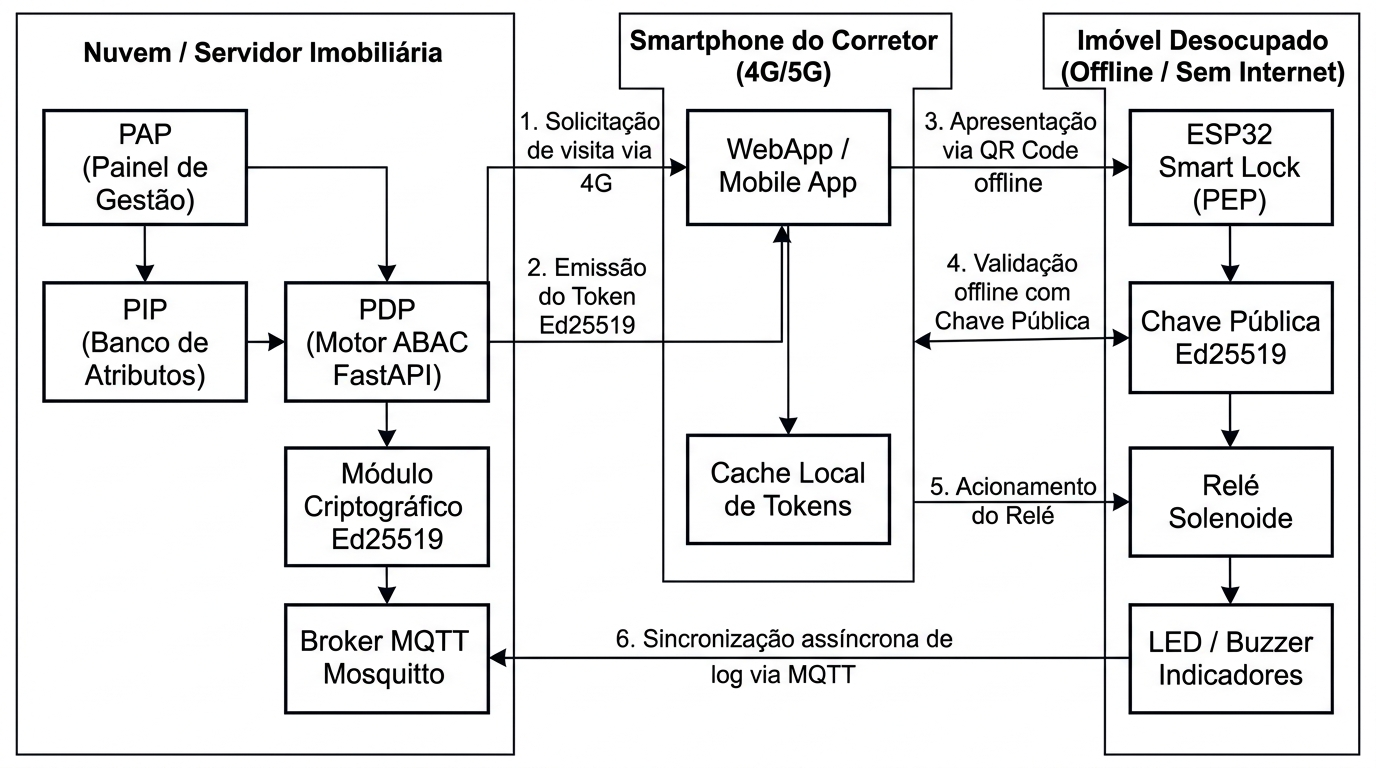
\includegraphics[width=0.92\textwidth]{imagens/01_arquitetura_visao_geral.jpg}
\fonte{Elaborado pelo autor (2026).}
\end{figure}

O ecossistema divide-se em três domínios físicos com responsabilidades bem delimitadas:

\begin{itemize}
    \item \textbf{Nuvem da Imobiliária:} Centraliza os serviços corporativos e a tomada de decisão. Contém o Painel de Gestão (\textit{Policy Administration Point} -- PAP), o repositório de atributos cadastrais (\textit{Policy Information Point} -- PIP), o motor de regras (\textit{Policy Decision Point} -- PDP em FastAPI), o módulo criptográfico detentor da chave privada Ed25519 e o broker MQTT (Eclipse Mosquitto) para recepção das telemetrias de auditoria.
    \item \textbf{Smartphone do Corretor:} Atua como elemento intermediário e portador (\textit{data mule/carrier}) de credenciais e telemetrias. Uma vez que o profissional dispõe de conectividade celular móvel (4G/5G), seu smartphone estabelece a ponte de comunicação entre a nuvem e o imóvel desocupado, requisitando o token pela internet e apresentando-o localmente por leitura óptica.
    \item \textbf{Nó da Fechadura (ESP32):} Atua como Ponto de Aplicação de Políticas (\textit{Policy Enforcement Point} -- PEP) local. Opera em regime estritamente desconectado (\textit{zero local infrastructure}), desprovido de conexão Wi-Fi ou modem celular. Armazena exclusivamente a chave pública da autoridade emissora em memória permanente protegida, garantindo que mesmo o acesso físico ao hardware não exponha segredos capazes de forjar credenciais.
\end{itemize}

O ciclo operacional entre esses domínios executa-se em seis etapas: (1) solicitação de visita via canal celular 4G/5G pelo aplicativo móvel; (2) avaliação de políticas no PDP e assinatura digital do token com a chave privada mestre Ed25519; (3) renderização da credencial em código QR dinâmico na tela do smartphone; (4) verificação determinística da assinatura no microcontrolador ESP32 contra a chave pública gravada no firmware; (5) comutação do relé por 5 segundos para retração do solenoide acompanhada de sinalização visual e sonora; e (6) despacho assíncrono do recibo de confirmação ao broker MQTT via smartphone sob QoS 1 (\textit{at least once}).

% ============================================================
\section{Modelo de Autorização Baseado em Atributos (ABAC)}
\label{sec:modelo-abac}
% ============================================================

\subsection{Transição do RBAC ao ABAC no Contexto Imobiliário}
\label{subsec:rbac-vs-abac}

O modelo de Controle de Acesso Baseado em Papéis (\textit{Role-Based Access Control} -- RBAC) restringe privilégios a partir de funções estáticas atribuídas a usuários. No cenário imobiliário, essa abordagem mostra-se insuficiente: determinar apenas que um indivíduo possui o papel de ``corretor'' não impede que ele ingresse na propriedade fora do horário comercial, acesse unidades vendidas ou entre em imóveis sem agendamento homologado. Tentar contornar essas limitações via RBAC gera explosão de papéis (\textit{role explosion}), tornando a administração impraticável.

O Controle de Acesso Baseado em Atributos (\textit{Attribute-Based Access Control} -- ABAC), adaptado da formulação HABAC$\alpha$ proposta por \citeonline{ameer2022}, soluciona essa restrição avaliando dinamicamente predicados lógicos em tempo de execução:

\begin{equation}
\label{eq:abac-decisao}
\text{Decisão} = f(U_{\text{atrib}},\; D_{\text{atrib}},\; OP_{\text{atrib}},\; ES_{\text{atrib}})
\end{equation}

Em que $U_{\text{atrib}}$ representa os atributos do sujeito solicitante, $D_{\text{atrib}}$ os atributos do dispositivo/imóvel de destino, $OP_{\text{atrib}}$ os parâmetros da ação requerida e $ES_{\text{atrib}}$ as variáveis contextuais do ambiente no instante da avaliação.

\subsection{Dicionário de Atributos do Sistema}
\label{subsec:dicionario-atributos}

O modelo formal implementado organiza treze atributos essenciais para a regulação do acesso às unidades, detalhados no Quadro~\ref{quadro:dicionario-atributos}.

\begin{table}[htbp]
\centering
\footnotesize
\caption{Dicionário de atributos do modelo ABAC projetado.}
\label{quadro:dicionario-atributos}
\begin{tabularx}{\textwidth}{cc p{4.2cm} X}
\toprule
\textbf{Entidade} & \textbf{Símbolo} & \textbf{Atributo} & \textbf{Definição e Tipagem} \\
\midrule
\multirow{4}{*}{Sujeito ($U$)} 
 & $U$ & \texttt{u.id} & String (UUID): Identificador único do corretor. \\
 & $U$ & \texttt{u.role} & Enum: \texttt{CORRETOR\_PARCEIRO}, \texttt{GESTOR}. \\
 & $U$ & \texttt{u.status} & Enum: \texttt{ATIVO}, \texttt{SUSPENSO}, \texttt{PENDENTE}. \\
 & $U$ & \texttt{u.device\_fp} & String (Hash SHA-256): Identificador do smartphone cadastrado. \\
\addlinespace
\multirow{3}{*}{Objeto ($D$)} 
 & $D$ & \texttt{d.lock\_id} & String (Hex): Identificador físico gravado no ESP32. \\
 & $D$ & \texttt{d.status\_imovel} & Enum: \texttt{DISPONIVEL\_VENDA}, \texttt{LOCADO}, \texttt{MANUTENCAO}. \\
 & $D$ & \texttt{d.lock\_state} & Enum: \texttt{TRAVADO}, \texttt{DESTRAVADO}, \texttt{BLOQUEIO}. \\
\addlinespace
\multirow{2}{*}{Ação ($OP$)} 
 & $OP$ & \texttt{op.tipo} & Enum: \texttt{SOLICITAR\_TOKEN}, \texttt{DESTRAVAR\_PORTA}. \\
 & $OP$ & \texttt{op.modo} & Enum: \texttt{OFFLINE\_BEARER}, \texttt{TELEMETRIA}. \\
\addlinespace
\multirow{4}{*}{Ambiente ($ES$)} 
 & $ES$ & \texttt{es.timestamp} & Inteiro (Unix Epoch): Horário de recepção da solicitação. \\
 & $ES$ & \texttt{es.horario\_comercial} & Booleano: \texttt{true} se horário atual estiver entre 08h e 19h. \\
 & $ES$ & \texttt{es.dia\_permitido} & Booleano: Restrição a finais de semana ou feriados. \\
 & $ES$ & \texttt{es.agendamento\_ativo} & Booleano: Confirmação de visita agendada na base imobiliária. \\
\bottomrule
\end{tabularx}
\fonte{Elaborado pelo autor (2026).}
\end{table}

\subsection{Arquitetura Funcional segundo o Padrão NIST SP 800-162}
\label{subsec:arquitetura-nist}

A segregação dos módulos de controle de acesso adota as especificações do padrão NIST SP 800-162, dividindo as responsabilidades de administração, persistência, inferência e aplicação, conforme exposto na Figura~\ref{fig:modelo-abac-nist}.

\begin{figure}[htbp]
\centering
\caption{Arquitetura funcional de controle de acesso ABAC baseada no padrão NIST SP 800-162.}
\label{fig:modelo-abac-nist}
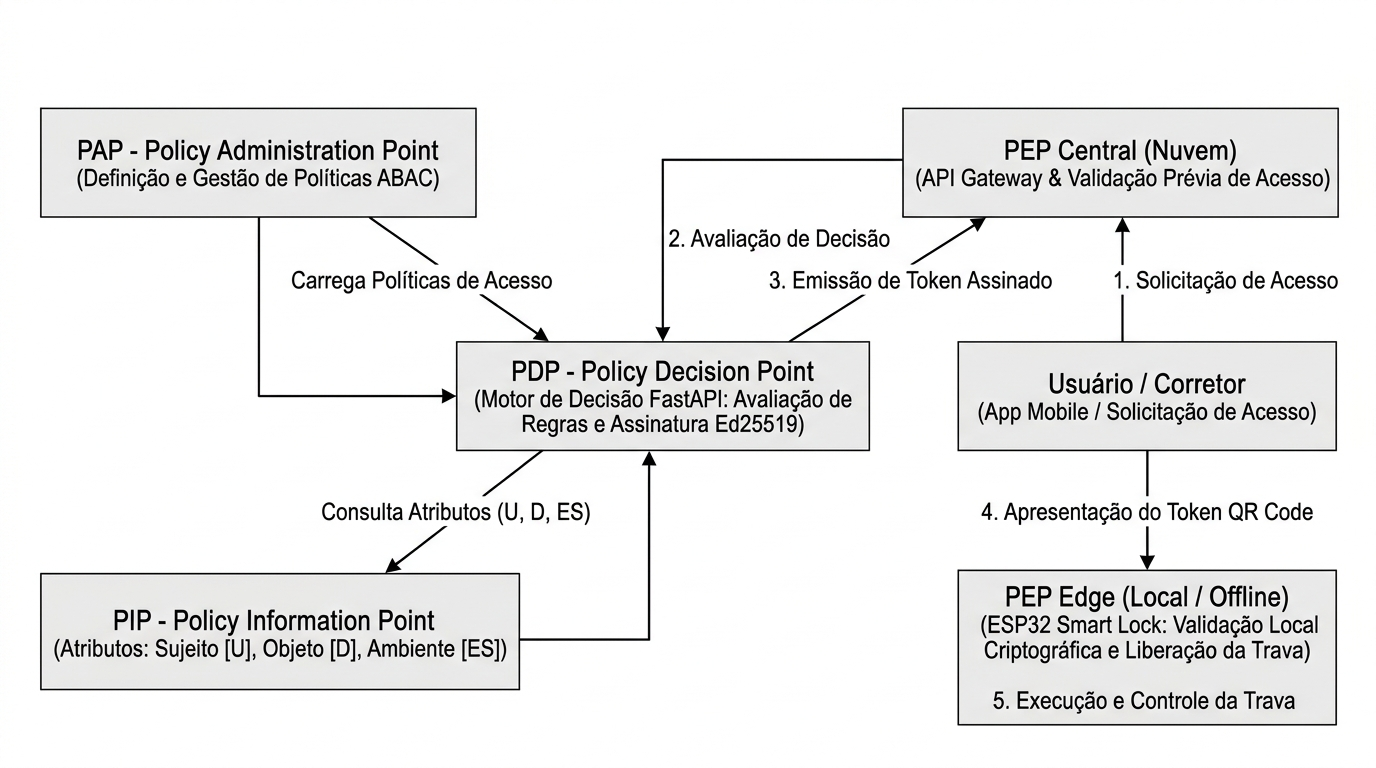
\includegraphics[width=0.78\textwidth, keepaspectratio]{imagens/03_modelo_abac_nist.jpg}
\fonte{Elaborado pelo autor (2026).}
\end{figure}

A interação entre os módulos ocorre de maneira estruturada:
\begin{itemize}
    \item \textbf{PAP (\textit{Policy Administration Point}):} Módulo administrativo em que gestores definem e atualizam as regras de visitação e horários permitidos.
    \item \textbf{PIP (\textit{Policy Information Point}):} Base relacional estruturada que fornece os valores correntes dos atributos vinculados ao usuário, à unidade imobiliária e à agenda.
    \item \textbf{PDP (\textit{Policy Decision Point}):} Motor de inferência construído sobre FastAPI/Python. Processa os dados da requisição, consulta o PIP, confronta as condições estipuladas na política e comanda o módulo criptográfico para emissão do token.
    \item \textbf{PEP Central (\textit{Cloud PEP}):} Ponto de aplicação no API Gateway de nuvem, responsável por barrar requisições malformadas ou com falha de autenticação preliminar.
    \item \textbf{PEP Borda (\textit{Edge PEP}):} Firmware embarcado no ESP32 na porta do imóvel. Recebe a credencial, checa a assinatura digital contra a chave pública e comuta o relé físico.
\end{itemize}

\subsection{Formalização das Regras de Acesso e Algoritmo de Combinação}
\label{subsec:regras-abac}

As políticas de acesso são estruturadas em formato JSON e avaliadas pelo PDP. O Código~\ref{lst:politica-abac} apresenta a regra fundamental aplicada às visitas de corretores parceiros.

\begin{lstlisting}[language=Python, caption={Estrutura da política de autorização ABAC implementada no PDP.}, label={lst:politica-abac}]
{
  "policy_id": "POL_VISITA_IMOVEL_DISPONIVEL",
  "description": "Permite visita de corretores ativos a imoveis disponiveis em horario comercial",
  "target": {
    "action": "SOLICITAR_TOKEN",
    "role": "CORRETOR_PARCEIRO"
  },
  "rules": [
    {
      "rule_id": "REGRA_01_STATUS_CORRETOR",
      "condition": "u.status == 'ATIVO'",
      "effect": "Permit"
    },
    {
      "rule_id": "REGRA_02_STATUS_IMOVEL",
      "condition": "d.status_imovel in ['DISPONIVEL_VENDA', 'DISPONIVEL_LOCACAO']",
      "effect": "Permit"
    },
    {
      "rule_id": "REGRA_03_JANELA_HORARIA",
      "condition": "es.horario_comercial == true and es.dia_permitido == true",
      "effect": "Permit"
    },
    {
      "rule_id": "REGRA_04_VINCULO_AGENDAMENTO",
      "condition": "es.agendamento_ativo == true",
      "effect": "Permit"
    }
  ],
  "rule_combining_algorithm": "deny_overrides"
}
\end{lstlisting}

O mecanismo adota a disciplina de combinação \texttt{deny\_overrides}: caso qualquer uma das regras retorne negação (\textit{Deny}), a requisição é sumariamente recusada pelo servidor, aplicando com rigor o princípio do privilégio mínimo.

% ============================================================
\section{Modelo Criptográfico e Validação Offline}
\label{sec:modelo-criptografico}
% ============================================================

\subsection{O Paradigma da Validação Desconectada (Analogia EMV)}
\label{subsec:analogia-emv}

O nó IoT instalado na porta opera sem conexão à internet no instante em que o corretor se apresenta no local. A concepção adotada baseia-se no princípio empregado pelo padrão bancário internacional EMV (\textit{Europay, Mastercard, Visa}) para transações em terminais desconectados (\textit{offline transaction verification}).

No padrão EMV, o terminal de pagamento não consulta o saldo em conta em tempo real, mas possui gravada a chave pública da autoridade emissora. Ao validar a assinatura digital contida no microprocessador do cartão, o terminal obtém garantia matemática de autenticidade da credencial e integridade dos dados da operação.

No artefato desenvolvido, o PDP na nuvem desempenha o papel de autoridade emissora, detendo a chave privada mestre. O smartphone atua como portador do token assinado. O microcontrolador ESP32 comporta-se de forma análoga ao terminal: a partir da chave pública armazenada em sua memória, autentica o token apresentado localmente sem recorrer a redes externas.

\subsection{Seleção do Algoritmo Criptográfico Ed25519}
\label{subsec:escolha-ed25519}

Microcontroladores de baixo consumo operam sob fortes restrições de memória volátil e capacidade aritmética. Algoritmos assimétricos tradicionais, como RSA-2048, exigem exponenciação modular pesada, demandando elevado tempo de processamento e consumo de memória RAM incompatível com o ESP32.

A criptografia de curvas elípticas contorna essa restrição. O algoritmo selecionado para o projeto foi o Ed25519 (\textit{Edwards-curve Digital Signature Algorithm}), baseado na Curva de Edwards Torcida Curve25519. O Quadro~\ref{quadro:comparativo-cripto} compara as características técnicas de esquemas comuns frente às demandas do nó embarcado.

\begin{table}[htbp]
\centering
\footnotesize
\caption{Comparativo entre esquemas criptográficos para validação em nós IoT embarcados.}
\label{quadro:comparativo-cripto}
\begin{tabularx}{\textwidth}{p{3.2cm} ccc X}
\toprule
\textbf{Critério} & \textbf{RSA-2048} & \textbf{HMAC-SHA256} & \textbf{Ed25519} & \textbf{Impacto no ESP32} \\
\midrule
Tipo de Chave & Assimétrica & Simétrica & Assimétrica & Protege contra cópia física da memória Flash. \\
Tamanho da Chave & 256 bytes & 32 bytes (segredo) & 32 bytes & Reduzida ocupação em memória permanente. \\
Tamanho da Assinatura & 256 bytes & 32 bytes & 64 bytes & Otimizado para pacotes seriais e códigos QR. \\
Tempo de Verificação & 150 a 300 ms & $<$ 1 ms & 1,8 a 3,5 ms & Desempenho quase instantâneo de abertura. \\
Nível de Segurança & 112 bits & 128 bits & 128 bits & Criptograficamente equivalente a RSA de 3072 bits. \\
Ataques de Canal Lateral & Moderada & Boa & Excelente & Imunidade a variações de tempo computacional. \\
\bottomrule
\end{tabularx}
\fonte{Elaborado pelo autor com base em \citeonline{ameer2022} e dados de literatura técnica (2026).}
\end{table}

A adoção do Ed25519 oferece uma vantagem estrutural: como o microcontrolador armazena exclusivamente a chave pública (32 bytes), mesmo que o equipamento seja subtraído fisicamente e sua memória extraída, nenhuma chave privada é comprometida, impedindo a geração forjada de credenciais para outras unidades.

\subsection{Estrutura do Token de Acesso}
\label{subsec:estrutura-token}

O token emitido pelo PDP é compactado em formato serializado JSON. O Código~\ref{lst:payload-token} ilustra a estrutura dos campos transmitidos.

\begin{lstlisting}[language=Python, caption={Estrutura formal do payload do token de acesso emitido pelo PDP.}, label={lst:payload-token}]
{
  "jti": "a7f4b892-91c2-4e88-9d21-f09b578c92a1",
  "sub": "corretor_id_8472",
  "dev": "lock_esp32_imovel_042",
  "nbf": 1774204800,
  "exp": 1774205700,
  "act": "UNLOCK_DOOR",
  "fp":  "e3b0c442...[hash SHA-256 do aparelho]...",
  "sig": "3a8f9c10...[64 bytes assinatura Ed25519]..."
}
\end{lstlisting}

O detalhamento funcional de cada parâmetro constituinte consta no Quadro~\ref{quadro:dicionario-token}.

\begin{table}[htbp]
\centering
\footnotesize
\caption{Dicionário de campos constituintes do token de acesso.}
\label{quadro:dicionario-token}
\begin{tabularx}{\textwidth}{p{1.4cm} p{2.8cm} X}
\toprule
\textbf{Campo} & \textbf{Nome Técnico} & \textbf{Finalidade Funcional} \\
\midrule
\texttt{jti} & JWT ID / Nonce & Identificador universal único (UUIDv4) para prevenção de ataques de repetição. \\
\texttt{sub} & \textit{Subject} & Identificador cadastral do corretor requerente habilitado. \\
\texttt{dev} & \textit{Device Target} & Identificador exclusivo da fechadura destinatária. Evita o uso em portas incorretas. \\
\texttt{nbf} & \textit{Not Before} & Timestamp Unix que estabelece o início da validade da permissão concedida. \\
\texttt{exp} & \textit{Expiration} & Timestamp Unix final de vigência (tempo de vida restrito a 15 minutos). \\
\texttt{act} & \textit{Action} & Ação delegada ao dispositivo físico (\texttt{UNLOCK\_DOOR}). \\
\texttt{fp} & \textit{Device Fingerprint} & Hash vinculado ao aparelho móvel cadastrado \cite{satanasaowapak2021}. \\
\texttt{sig} & \textit{Digital Signature} & Assinatura de 64 bytes gerada pelo PDP com a chave privada mestre Ed25519. \\
\bottomrule
\end{tabularx}
\fonte{Elaborado pelo autor (2026).}
\end{table}

\subsection{Algoritmo de Verificação Local no ESP32}
\label{subsec:algoritmo-verificacao-esp32}

Ao receber o payload serial via interface de leitura, o firmware do ESP32 processa os dados por meio de uma bateria determinística de cinco testes, conforme sumarizado na Figura~\ref{fig:fluxo-validacao-offline}.

\begin{figure}[htbp]
\centering
\caption{Fluxograma de validação determinística de tokens offline no microcontrolador ESP32.}
\label{fig:fluxo-validacao-offline}
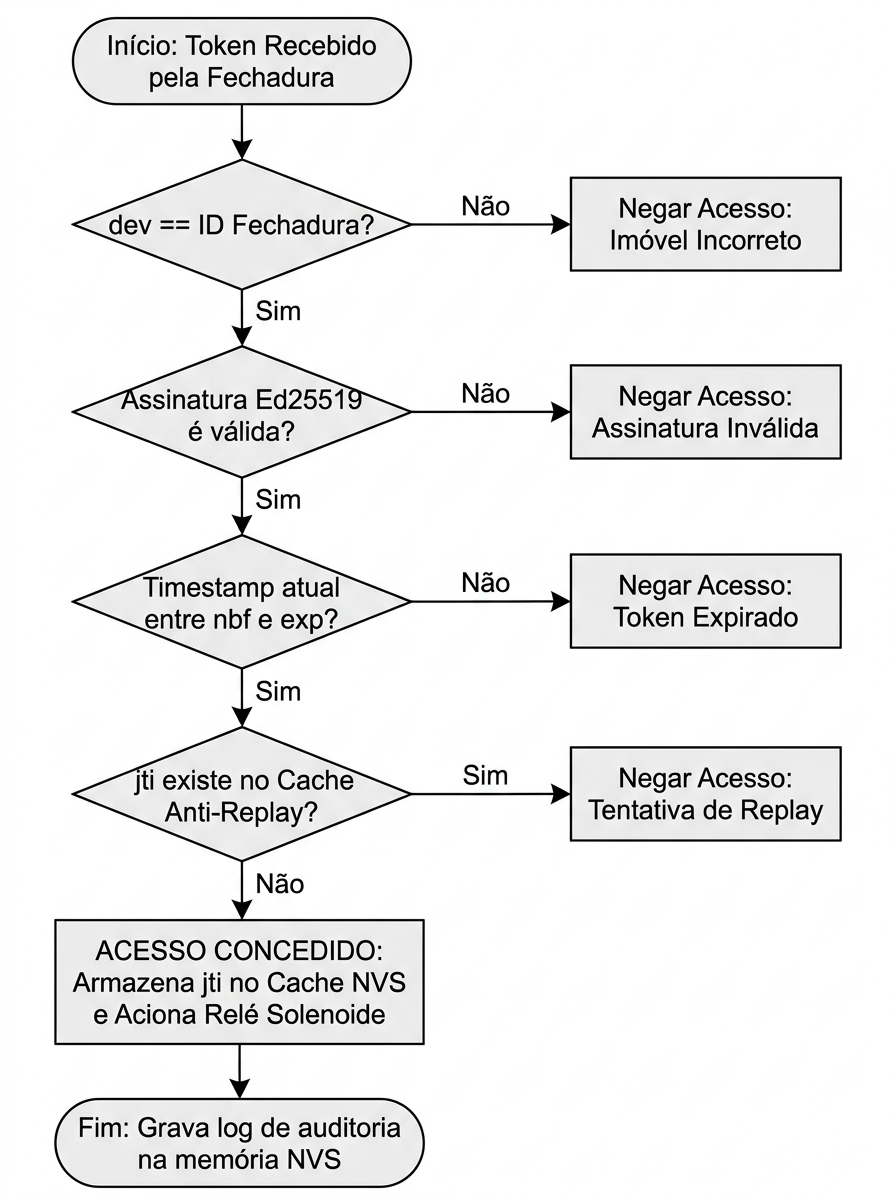
\includegraphics[width=0.88\textwidth]{imagens/02_fluxo_validacao_offline.jpg}
\fonte{Elaborado pelo autor (2026).}
\end{figure}

O fluxo executa-se com término antecipado ao menor indício de inconsistência:
\begin{enumerate}
    \item \textbf{Verificação de Destino (\texttt{dev}):} Compara o campo \texttt{dev} com a identidade física da fechadura gravada na partição de configuração.
    \item \textbf{Verificação Criptográfica (\texttt{sig}):} Invoca a biblioteca \texttt{mbedtls} para recalcular a verificação assimétrica da assinatura com a chave pública mestre.
    \item \textbf{Verificação Temporal (\texttt{nbf} e \texttt{exp}):} Compara o horário interno com a janela permitida.
    \item \textbf{Verificação de Unicidade (\texttt{jti}):} Consulta a partição NVS para checar se o token já foi consumido.
    \item \textbf{Atuação Mecânica:} Persiste o \texttt{jti} no buffer histórico, aciona o relé por 5 segundos e ativa a sinalização audiovisual.
\end{enumerate}

\subsection{Prevenção contra Ataques e Gestão do Buffer Anti-Replay}
\label{subsec:anti-replay}

Para assegurar que interceptações não permitam aberturas indevidas, o sistema projeta as contramedidas estruturadas no Quadro~\ref{quadro:vetores-ataque}.

\begin{table}[htbp]
\centering
\footnotesize
\caption{Matriz de contramedidas de segurança projetadas contra vetores de ataque.}
\label{quadro:vetores-ataque}
\begin{tabularx}{\textwidth}{p{3cm} X p{5.2cm}}
\toprule
\textbf{Vetor de Ataque} & \textbf{Descrição do Ataque} & \textbf{Mecanismo de Defesa do Artefato} \\
\midrule
Replay Attack & Interceptação do código QR para reapresentação posterior ao leitor. & O \texttt{jti} é gravado em buffer circular na memória Flash NVS. Reenvios são barrados. \\
Token Expirado & Uso de credencial legítima após o horário autorizado. & Confronto do timestamp \texttt{exp} com descarte de tokens com TTL estourado. \\
Adulteração de Payload & Tentativa de forjar horário de término ou trocar identificador de imóvel. & A assinatura Ed25519 é invalidada matematicamente; leitura é recusada. \\
Imóvel Incorreto & Uso de token da Unidade A na Unidade B. & O identificador \texttt{dev} diverge da identidade estática da fechadura. \\
Compartilhamento & Envio de captura de tela para terceiro não credenciado. & O hash \texttt{fp} vincula o token ao smartphone registrado \cite{satanasaowapak2021}. \\
Subtração do Nó & Furto físico do dispositivo para clonagem de chaves. & O microcontrolador guarda apenas a chave pública; chaves privadas ficam isoladas na nuvem. \\
\bottomrule
\end{tabularx}
\fonte{Elaborado pelo autor (2026).}
\end{table}

A gestão do buffer anti-replay dimensiona uma fila circular na memória flash NVS com capacidade para reter até 200 identificadores \texttt{jti}. Com validade restrita a 15 minutos (900 segundos) por token, o buffer de 200 posições atende com margem à rotina de visitas, ocupando menos de 8~KB na partição de dados.

% ============================================================
\section{Fluxo de Operação de Ponta a Ponta}
\label{sec:fluxo-ponta-a-ponta}
% ============================================================

A operação do ecossistema divide-se em três etapas coordenadas: emissão online do token pela nuvem, validação local offline no imóvel e sincronização assíncrona de auditoria. A Figura~\ref{fig:diagrama-sequencia-visita} expõe o diagrama de sequência detalhado.

\begin{figure}[htbp]
\centering
\caption{Diagrama de sequência ponta a ponta do processo de requisição, validação e auditoria de visitas.}
\label{fig:diagrama-sequencia-visita}
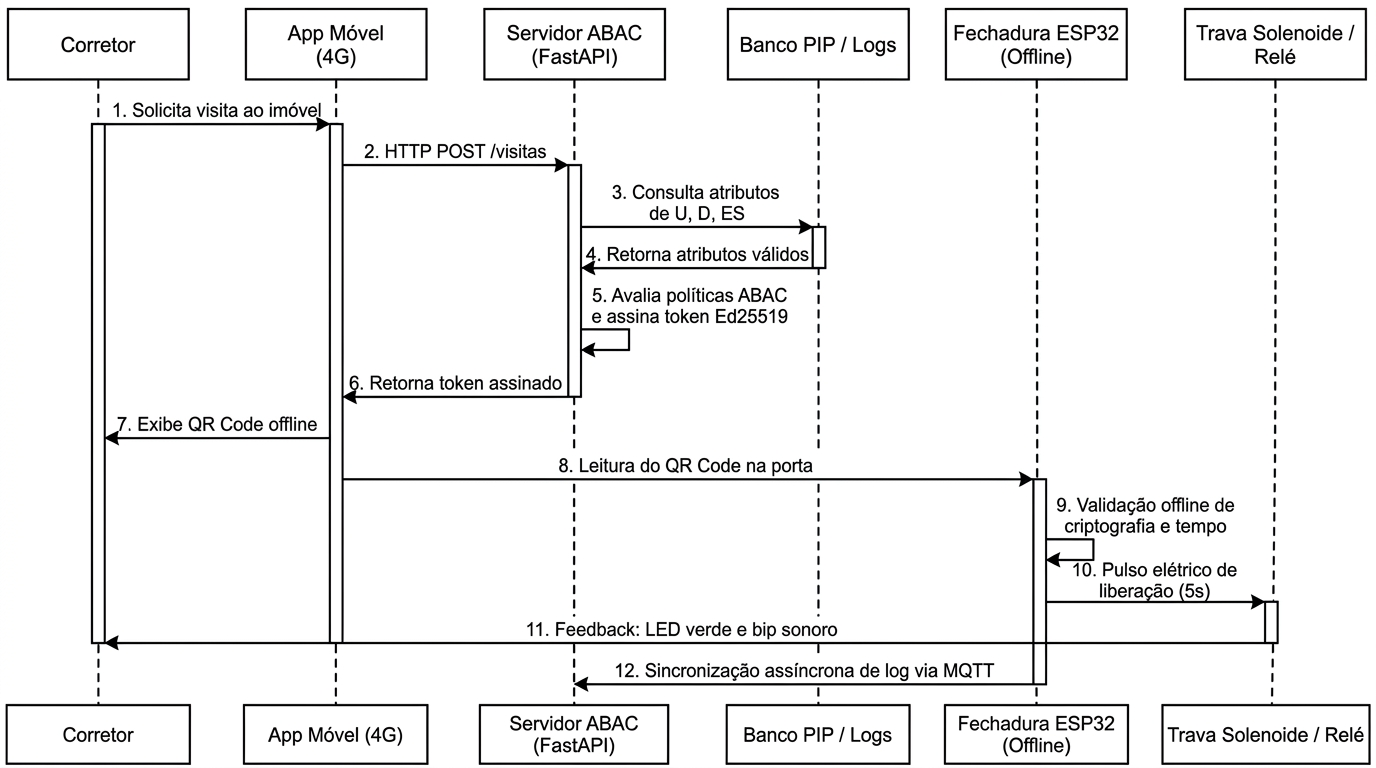
\includegraphics[width=0.95\textwidth]{imagens/04_diagrama_sequencia_visita.jpg}
\fonte{Elaborado pelo autor (2026).}
\end{figure}

\subsection{Fase 1: Solicitação e Emissão do Token (Online)}
\label{subsec:fluxo-fase-emissao}

\begin{enumerate}
    \item Ao se aproximar do imóvel, o corretor aciona o aplicativo em seu smartphone conectado à rede celular (4G/5G).
    \item O aplicativo envia uma requisição HTTP via TLS pelo endpoint \path{/api/v1/access/request-token} ao servidor central, informando suas credenciais, identificador do imóvel e assinatura digital do aparelho móvel.
    \item O PDP recebe a requisição e interroga o banco relacional (PIP) para obter a situação cadastral do corretor, regras do condomínio e agendamento ativo.
    \item O motor ABAC processa as condições declaradas na política ativa.
    \item Havendo conformidade, o módulo criptográfico gera o payload com identificador \texttt{jti} inédito, calcula a assinatura digital com a chave privada mestre Ed25519 e devolve o pacote codificado em JSON sob código HTTP 200. Havendo inconformidade, o servidor devolve código HTTP 403 com a justificativa de negação.
    \item O aplicativo retém a credencial em cache seguro e gera na tela um código QR dinâmico com o payload serializado.
\end{enumerate}

\subsection{Fase 2: Apresentação e Validação Local (Offline)}
\label{subsec:fluxo-fase-validacao}

\begin{enumerate}
    \item O corretor aproxima a tela do smartphone da interface de leitura associada ao microcontrolador ESP32 na porta do imóvel.
    \item O microcontrolador processa a cadeia de caracteres recebida e reconstrói o payload em memória de trabalho.
    \item O firmware executa a rotina de validação: confere o código \texttt{dev}, verifica a assinatura Ed25519 com a chave pública instalada, atesta a janela de vigência (\texttt{nbf} e \texttt{exp}) e busca o \texttt{jti} no buffer anti-replay.
    \item Comprovada a autenticidade e tempestividade do token, o pino GPIO 23 é levado a nível lógico alto, excitando a bobina do relé por 5 segundos para retração do pino solenoide. Concomitantemente, o LED verde (GPIO 2) acende e o \textit{buzzer} (GPIO 18) emite um sinal agudo.
    \item O identificador \texttt{jti} é gravado na memória Flash NVS local.
\end{enumerate}

\subsection{Fase 3: Sincronização Assíncrona e Auditoria}
\label{subsec:fluxo-fase-auditoria}

\begin{enumerate}
    \item Concluída a abertura física, o aplicativo do corretor gera um recibo assinado contendo o \texttt{jti} consumido e o timestamp da operação.
    \item O smartphone despacha o recibo ao broker MQTT corporativo (Eclipse Mosquitto) no canal \texttt{imobiliaria/auditoria/acessos}, via conexão celular e nível de serviço QoS 1 (\textit{at least once}).
    \item O serviço de auditoria em nuvem armazena a mensagem na base relacional da imobiliária, garantindo rastreabilidade sem violar o isolamento do nó físico.
\end{enumerate}

% ============================================================
\section{Stack Tecnológica e Especificação do Firmware}
\label{sec:stack-tecnologica}
% ============================================================

\subsection{Mapeamento dos Componentes Tecnológicos}
\label{subsec:mapeamento-stack}

A escolha das ferramentas orientou-se pela padronização acadêmica e viabilidade de execução em sistemas embarcados restritos. O Quadro~\ref{quadro:stack-tecnologica} sintetiza os componentes da solução.

\begin{table}[htbp]
\centering
\footnotesize
\caption{Mapeamento da pilha tecnológica empregada no desenvolvimento do artefato.}
\label{quadro:stack-tecnologica}
\begin{tabularx}{\textwidth}{p{2.8cm} p{4.2cm} X}
\toprule
\textbf{Camada / Módulo} & \textbf{Tecnologia Selecionada} & \textbf{Justificativa Técnica e Acadêmica} \\
\midrule
Nó da Fechadura (PEP) & ESP32 DevKit v1 (Xtensa LX6 Dual-Core 240 MHz) & Plataforma consolidada na literatura de automação e segurança IoT residencial \cite{vardakis2024}. \\
Linguagem do Firmware & C/C++ sobre PlatformIO / Framework Arduino & Controle determinístico de memória e integração nativa à biblioteca criptográfica \texttt{mbedtls}. \\
Servidor de Políticas (PDP) & Python 3.11+ com FastAPI & Arquitetura assíncrona ASGI de alto rendimento, tipagem estrita com Pydantic e documentação OpenAPI. \\
Biblioteca Criptográfica & PyNaCl (Servidor) e mbedtls (ESP32) & Implementações de referência do algoritmo Ed25519 resistentes a vazamento por canal lateral. \\
Broker de Mensageria & Eclipse Mosquitto v2.0+ & Padrão aberto com suporte nativo a MQTT v3.1.1/v5.0, baixo consumo de memória ($<$ 10~MB) e garantia QoS 1. \\
Ambiente de Simulação & Wokwi IoT Simulator & Plataforma com emulação precisa de registradores do ESP32, suporte a rede virtual e periféricos. \\
Interface do Corretor & Progressive Web App (PWA) em HTML5/JS & Permite acesso multiplataforma via navegador móvel sem fricção de distribuição em lojas de aplicativos. \\
Ferramentas de Carga & Locust e Pytest & Automação de testes de estresse, injeção de requisições concorrentes e mensuração de latências. \\
\bottomrule
\end{tabularx}
\fonte{Elaborado pelo autor (2026).}
\end{table}

\subsection{Organização Modular do Firmware no ESP32}
\label{subsec:modulos-firmware}

O software a ser embarcado no microcontrolador organiza-se em três módulos desacoplados:

\begin{description}
    \item[\texttt{crypto\_verifier.cpp}:] Isola o subsistema criptográfico. Contém a chave pública mestre de 32 bytes (\texttt{SERVER\_PUBLIC\_KEY}) gravada em memória de programa (\texttt{PROGMEM}). Inicializa as estruturas da biblioteca \texttt{mbedtls} e disponibiliza a função \texttt{verify\_ed25519\_signature(payload, signature, pubkey)}.
    \item[\texttt{token\_validator.cpp}:] Executa a análise semântica dos dados recebidos. Utiliza a biblioteca \texttt{ArduinoJson} com alocação estática de memória (\texttt{StaticJsonDocument}) para prevenir fragmentação de heap. Realiza o confronto do campo \texttt{dev}, checagem de janelas temporais e iteração sobre a lista anti-replay mantida na NVS.
    \item[\texttt{lock\_actuator.cpp}:] Gerencia a interface com atuadores e sinalizadores físicos. Controla os estados dos pinos GPIO por temporizadores não bloqueantes baseados na função \texttt{millis()}, eliminando bloqueios de processamento.
\end{description}

\subsection{Endpoints e Motor de Inferência em FastAPI}
\label{subsec:endpoints-api}

O backend construído sobre FastAPI disponibiliza três pontos de entrada principais:

\begin{itemize}
    \item \texttt{POST /api/v1/access/request-token}: Endpoint principal de requisição. Recebe as credenciais do corretor, ID do imóvel e dados contextuais. Aciona a função de inferência ABAC, consulta a base relacional e, havendo decisão afirmativa, emprega o método \texttt{crypto\_sign\_detached} da biblioteca \texttt{PyNaCl} para produzir a assinatura do token.
    \item \texttt{PATCH /api/v1/corretores/\{id\}/status}: Ponto de gestão cadastral utilizado por administradores. Permite alterar o status de um corretor de \texttt{ATIVO} para \texttt{SUSPENSO}. Modificações refletem-se instantaneamente no banco relacional, bloqueando emissões subsequentes de tokens.
    \item \texttt{GET /api/v1/imoveis/\{id\}/logs}: Consulta a série histórica de acessos registrados para uma determinada unidade imobiliária, viabilizando relatórios gerenciais de auditoria.
\end{itemize}

\subsection{Estrutura de Mensageria e Tópicos MQTT}
\label{subsec:topicos-mqtt}

Para garantir a rastreabilidade dos eventos, as mensagens transitam pelo broker Eclipse Mosquitto estruturadas sob uma hierarquia padronizada de tópicos:

\begin{lstlisting}[language=bash, caption={Estrutura hierárquica de tópicos MQTT empregada no sistema.}, label={lst:topicos-mqtt}]
imobiliaria/
+-- imoveis/{imovel_id}/
|   +-- status          # Telemetria: Online/Offline/Bateria
|   +-- revogacoes      # Broadcast de revogacao emergencial
|   +-- telemetria      # Tempo de resposta e diagnosticos
+-- auditoria/
|   +-- acessos         # Recibos de acessos executados
|   +-- alertas         # Tentativas com token invalido
+-- comandos/{imovel_id}/
    +-- emergencia      # Bloqueio forcado administrativo
\end{lstlisting}

O pacote de auditoria remetido ao canal \texttt{imobiliaria/auditoria/acessos} adota a estrutura esquemática apresentada no Código~\ref{lst:pacote-auditoria}.

\begin{lstlisting}[language=Python, caption={Formato esquemático do pacote de auditoria despachado via MQTT QoS 1.}, label={lst:pacote-auditoria}]
{
  "event_id": "evt_998124_ack",
  "timestamp": 1774204850,
  "imovel_id": "lock_esp32_imovel_042",
  "corretor_id": "corretor_id_8472",
  "jti_utilizado": "a7f4b892-91c2-4e88-9d21-f09b578c92a1",
  "resultado": "ACESSO_CONCEDIDO",
  "latencia_validacao_ms": 2.45,
  "latencia_comunicacao_ms": 178.30
}
\end{lstlisting}

% ============================================================
\section{Bancada de Simulação Virtual no Wokwi}
\label{sec:bancada-simulacao}
% ============================================================

\subsection{Mapeamento do Circuito Eletrônico e Pinout}
\label{subsec:circuito-wokwi}

O circuito virtual foi modelado no Wokwi Simulator utilizando o módulo virtual ESP32 DevKit v1. As ligações elétricas aos periféricos virtuais utilizam o mapa de pinos indicado no Quadro~\ref{quadro:pinout-esp32}.

\begin{table}[htbp]
\centering
\footnotesize
\caption{Mapeamento dos pinos GPIO e periféricos no circuito virtual ESP32.}
\label{quadro:pinout-esp32}
\begin{tabularx}{\textwidth}{c c p{3.8cm} X}
\toprule
\textbf{Pino GPIO} & \textbf{Direção} & \textbf{Dispositivo Conectado} & \textbf{Comportamento e Função} \\
\midrule
GPIO 23 & Saída (Digital) & Módulo Relé Solenoide & Nível ALTO comuta o relé por 5 segundos para liberar a trava. \\
GPIO 2 & Saída (Digital) & LED Verde & Pulso luminoso que indica validação e liberação do acesso. \\
GPIO 4 & Saída (Digital) & LED Vermelho & Sinaliza rejeição (token inválido, expirado ou unidade divergente). \\
GPIO 18 & Saída (PWM) & Buzzer Piezoelétrico & Emite um tom agudo para sucesso e dois graves para rejeição. \\
GPIO 16 / 17 & Entrada/Saída & Porta Serial / Leitor RX/TX & Recepção dos dados brutos correspondentes à leitura do código. \\
\bottomrule
\end{tabularx}
\fonte{Elaborado pelo autor (2026).}
\end{table}

A topologia das conexões entre pinos, componentes e referências de terra (GND) é parametrizada no arquivo descritivo \texttt{diagram.json}, reproduzido no Código~\ref{lst:diagram-wokwi}.

\begin{lstlisting}[language=Python, caption={Arquivo descritivo diagram.json do circuito virtual no simulador Wokwi.}, label={lst:diagram-wokwi}]
{
  "version": 1,
  "author": "Controle de Acesso IoT - TCC",
  "editor": "wokwi",
  "parts": [
    { "type": "wokwi-esp32-devkit-v1", "id": "esp", "top": 0, "left": 0, "attrs": {} },
    { "type": "wokwi-relay-module", "id": "relay", "top": 100, "left": 150, "attrs": {} },
    { "type": "wokwi-led", "id": "led_green", "top": -50, "left": 120, "attrs": { "color": "green" } },
    { "type": "wokwi-led", "id": "led_red", "top": -50, "left": 160, "attrs": { "color": "red" } },
    { "type": "wokwi-buzzer", "id": "buzzer", "top": -50, "left": 200, "attrs": {} }
  ],
  "connections": [
    [ "esp:TX", "relay:IN", "green", [ "h20", "v40" ] ],
    [ "esp:D2", "led_green:A", "green", [ "h10", "v-30" ] ],
    [ "esp:D4", "led_red:A", "red", [ "h10", "v-30" ] ],
    [ "esp:D18", "buzzer:2", "blue", [ "h10", "v-30" ] ],
    [ "esp:GND.1", "relay:GND", "black", [ "h0" ] ],
    [ "esp:GND.1", "led_green:C", "black", [ "h0" ] ],
    [ "esp:GND.1", "led_red:C", "black", [ "h0" ] ],
    [ "esp:GND.1", "buzzer:1", "black", [ "h0" ] ]
  ]
}
\end{lstlisting}

% ============================================================
\section{Comportamentos Esperados nos Cenários de Demonstração}
\label{sec:resultados-demonstracao}
% ============================================================

Em alinhamento com a etapa de demonstração da DSR e os objetivos específicos do projeto, estruturam-se os comportamentos projetados para os três cenários operacionais que serão submetidos a ensaios em bancada virtual.

\subsection{Cenário 1: Comportamento Esperado no Fluxo Nominal}
\label{subsec:res-cenario-1}

No fluxo nominal, prevê-se que o corretor com cadastro ativo requisite a entrada para um imóvel disponível dentro do horário comercial e com agendamento homologado.

Espera-se que o motor ABAC (PDP) execute a inferência lógica em tempo reduzido ($< 50$~ms) e invoque o módulo criptográfico para assinatura Ed25519 ($< 5$~ms). Ao apresentar o código QR renderizado na tela do celular à interface óptica do ESP32 na bancada simulada, o comportamento projetado consiste em:
\begin{enumerate}
    \item Conclusão da verificação matemática da assinatura digital em menos de 10~ms;
    \item Comutação do pino GPIO 23 para nível lógico alto por exatamente 5 segundos, acionando a bobina do relé solenoide;
    \item Acendimento do LED verde de confirmação e emissão de pulso agudo no buzzer;
    \item Transmissão assíncrona bem-sucedida do recibo de confirmação pelo aplicativo celular ao broker MQTT, sem perda de pacotes sob QoS 1.
\end{enumerate}

\subsection{Cenário 2: Comportamento Esperado frente a Acessos Inválidos e Ataques}
\label{subsec:res-cenario-2}

Para os ensaios negativos previstos (CT-2.1 a CT-2.4), a hipótese central de segurança requer uma taxa de contenção de 100\% de bloqueio efetivo na extremidade desconectada, sem qualquer falso positivo de concessão:

\begin{itemize}
    \item \textbf{CT-2.1 (Token Expirado):} Diante de tokens com timestamp posterior ao campo \texttt{exp}, espera-se que o firmware efetue o descarte imediato por estouro de TTL, acionando o LED vermelho (GPIO 4) e registrando a tentativa no log local sem comutação do relé.
    \item \textbf{CT-2.2 (Imóvel Divergente):} Caso um token emitido para a Unidade A seja apresentado na fechadura da Unidade B, espera-se que a checagem do campo \texttt{dev} falhe no primeiro estágio algorítmico, bloqueando o processamento antes mesmo da computação criptográfica.
    \item \textbf{CT-2.3 (Assinatura Forjada por Adulteração de Payload):} Diante de adulterações intencionais de bits em campos como vigência ou identificador de usuário, espera-se que a função \texttt{verify\_ed25519} retorne falso deterministicamente, impedindo a liberação física da porta.
    \item \textbf{CT-2.4 (Ataque de Repetição / \textit{Replay}):} Caso uma credencial consumida anteriormente seja apresentada de forma reincidente, espera-se que a rotina de busca na tabela circular NVS identifique a presença do identificador \texttt{jti}, barrando o acesso por duplicidade.
\end{itemize}

\subsection{Cenário 3: Comportamento Esperado na Revogação Cadastral}
\label{subsec:res-cenario-3}

Para a hipótese de revogação cadastral de um corretor na imobiliária, o comportamento projetado divide-se em duas respostas coordenadas:

No ambiente em nuvem, projeta-se que a alteração do status para \texttt{SUSPENSO} reflita de forma imediata no banco relacional (PIP). Requisições subsequentes submetidas pelo aplicativo devem ser indeferidas pelo PDP com código HTTP 403 (\textit{Forbidden}), impedindo a emissão de novos tokens.

No nó da fechadura desconectado, o controle do risco residual decorrente de credenciais geradas instantes antes da suspensão deve ser contido pela expiração temporal intrínseca: o token permanecerá operável apenas durante o intervalo remanescente de seu tempo de vida (TTL máximo de 15 minutos). Esgotada essa janela, o relógio interno do microcontrolador rejeitará o token por expiração, ao passo que tentativas de reuso dentro da janela serão inviabilizadas pelo mecanismo anti-replay.

% ============================================================
\section{Resultados Esperados e Discussão de Hipóteses}
\label{sec:analise-quantitativa}
% ============================================================

Em consonância com o protocolo experimental planejado na metodologia, estabelecem-se as metas de desempenho e as hipóteses analíticas que balizarão a coleta de dados durante os ensaios práticos.

\subsection{Hipóteses de Desempenho Temporal e Latência}
\label{subsec:res-desempenho-temporal}

A avaliação temporal contempla quatro métricas em cadeia: o tempo de decisão das políticas ABAC (M1), o tempo de cálculo da assinatura assimétrica Ed25519 no servidor (M2), o tempo de verificação matemática da assinatura no microcontrolador ESP32 (M3) e o tempo total de resposta perceptível pelo usuário (M4).

Para a inferência ABAC (M1), a meta de tempo médio inferior a 50~ms apoia-se em estudos prévios de motores de políticas contextuais. \citeonline{ameer2022} observaram tempos de decisão entre 15 e 40~ms para regras HABAC em servidores de aplicação. Como a implementação utiliza o framework assíncrono FastAPI (ASGI) associado a consultas indexadas no banco relacional (PIP), o limite de 50~ms garante que a avaliação das políticas lógicas sob a disciplina \texttt{deny\_overrides} ocorra sem bloqueio de threads de I/O.

Para a assinatura digital no servidor (M2), a meta de tempo inferior a 5~ms decorre das características computacionais da Curva de Edwards. Utilizando a biblioteca \texttt{PyNaCl} (baseada na implementação de referência \texttt{libsodium} em C), operações com o algoritmo Ed25519 em processadores de servidor x86-64 consomem tipicamente entre 0,05 e 1,5~ms \cite{hanblockchainoffline2018}. A margem de 5~ms absorve variações sob concorrência de requisições sem degradar a capacidade de resposta do backend.

Na extremidade desconectada, a verificação da assinatura Ed25519 no microcontrolador ESP32 a 240~MHz (M3) tem como meta estrita um tempo inferior a 10~ms. Essa delimitação ganha relevância quando confrontada com esquemas criptográficos tradicionais: \citeonline{hanotmpp2l2020} mediram uma latência de 339~ms para verificação assimétrica baseada em RSA-2048 em um microprocessador ARM Cortex-A7, atraso já perceptível ao usuário. No ESP32, a multiplicação de ponto na curva Curve25519 via biblioteca \texttt{mbedtls} consome menos de 800.000 ciclos de clock (cerca de 2 a 3,5~ms a 240~MHz). O teto de 10~ms fornece margem segura para trocas de contexto no FreeRTOS, garantindo que o destravamento ocorra de forma quase instantânea na porta.

Para a latência total ponta a ponta (M4) --- englobando tráfego de rede celular 4G/5G (150 a 250~ms), inferência em nuvem M1+M2 ($<$ 55~ms), leitura óptica do QR Code e verificação local M3 ($<$ 10~ms) ---, a meta fixada é inferior a 500~ms. Esse patamar apoia-se em diretrizes clássicas de ergonomia computacional (limite de 1 segundo para manutenção do fluxo contínuo de pensamento sem percepção de lentidão) e nas conclusões de \citeonline{satanasaowapak2021} sobre o tempo aceitável em fechaduras inteligentes residenciais.

\subsection{Restrições e Consumo de Recursos Computacionais no ESP32}
\label{subsec:res-consumo-recursos}

Em nós embarcados que operam de forma isolada, a gestão de memória determina a estabilidade operacional contínua. A métrica M5 estabelece que o consumo de memória RAM Heap no ESP32 não ultrapasse 120~KB durante o pico de decodificação JSON e verificação criptográfica. Fisicamente, o ESP32 dispõe de 520~KB de SRAM interna, dos quais aproximadamente 280 a 300~KB permanecem utilizáveis pela aplicação após a carga do FreeRTOS e pilhas nativas. O teto de 120~KB assegura que o firmware ocupe menos de 40\% da memória dinâmica disponível, mantendo margem livre contínua superior a 150~KB. Essa folga, associada à alocação estática com a biblioteca \texttt{ArduinoJson} (\texttt{StaticJsonDocument}), previne fragmentação de heap e falhas por estouro de memória (\textit{Out-Of-Memory}) \cite{vardakis2024}.

Para a memória permanente Flash ROM (M6), a meta restringe a ocupação do binário a menos de 35\% da partição de aplicação. O ESP32 DevKit v1 padrão integra 4~MB (4.096~KB) de memória Flash SPI. Em arquiteturas embarcadas de produção, adota-se o esquema de particionamento duplo para atualizações remotas seguras (\textit{Over-The-Air} -- OTA), no qual existem duas partições de aplicação espelhadas (\texttt{app0} e \texttt{app1}) com cerca de 1.300 a 1.400~KB cada (~32\% a 35\% da flash total). Manter o binário estático abaixo de 35\% é um requisito técnico mandatório para assegurar a viabilidade de atualização e mecanismos de recuperação automática (\textit{rollback}) \cite{simperf2024}.

\subsection{Capacidade de Mensageria e Eficácia de Segurança Projetada}
\label{subsec:res-vazao-seguranca}

Para a métrica M7, a meta de suportar mais de 100 mensagens por segundo no broker Eclipse Mosquitto decorre do dimensionamento de pico de administradoras imobiliárias de médio e grande porte. Mesmo em carteiras com centenas de propriedades e dezenas de corretores ativos em campo nos horários de maior visitação (início da tarde e finais de semana), a taxa de check-ins concorrentes raramente atinge dezenas de acessos por segundo. Como o broker Mosquitto foi desenvolvido em linguagem C com arquitetura assíncrona leve \cite{shauto2024}, a meta de 100 msg/s sob entrega garantida QoS 1 assegura uma margem de folga de cinco a dez vezes sobre o tráfego estimado, sem risco de enfileiramento ou descarte de pacotes de auditoria \cite{ameer2022}.

Por fim, a métrica M8 exige 100\% de bloqueio efetivo frente a tentativas anômalas (CT-2.1 a CT-2.4). Em controle de acesso físico a propriedades desocupadas, a tolerância a falsos positivos de concessão é zero. A fundamentação é matemática: a verificação de assinatura digital sobre curvas de Edwards é uma operação determinística estrita; qualquer alteração de um único bit no payload serializado invalida a prova criptográfica, forçando o algoritmo a retornar falso. Aliado ao buffer circular na partição NVS que impede a reutilização de identificadores \texttt{jti}, o sistema garante a rejeição categórica de acessos expirados, adulterados ou duplicados \cite{satanasaowapak2021}.

\subsection{Quadro Consolidado de Metas e Resultados Esperados}
\label{subsec:quadro-consolidado-resultados}

O Quadro~\ref{quadro:resultados-experimentais} consolida as variáveis de avaliação, as metas numéricas projetadas, os critérios de tolerância e a fundamentação teórica de cada parâmetro a ser aferido nas baterias de 50 repetições.

\begin{table}[htbp]
\centering
\footnotesize
\caption{Quadro consolidado de metas quantitativas e resultados esperados da avaliação experimental.}
\label{quadro:resultados-experimentais}
\begin{tabularx}{\textwidth}{c p{3.6cm} c p{3.2cm} X}
\toprule
\textbf{\#} & \textbf{Variável / Métrica} & \textbf{Meta} & \textbf{Critério de Aceitação} & \textbf{Fundamentação Teórica na Literatura} \\
\midrule
M1 & Latência Decisão ABAC (ms) & $<$ 50 & Ausência de bloqueios de thread no servidor. & Arquitetura assíncrona ASGI/FastAPI com regras JSON compiladas \cite{ameer2022}. \\
\addlinespace
M2 & Assinatura Ed25519 (ms) & $<$ 5 & Execução em tempo constante sem canal lateral. & Operação algébrica otimizada da biblioteca PyNaCl/libsodium \cite{hanblockchainoffline2018}. \\
\addlinespace
M3 & Verificação no ESP32 (ms) & $<$ 10 & Operação matemática instantânea no microcontrolador. & Desempenho de curvas elípticas Curve25519 a 240~MHz via \texttt{mbedtls} \cite{simperf2024}. \\
\addlinespace
M4 & Latência Ponta a Ponta (ms) & $<$ 500 & Tempo total imperceptível ao usuário na porta. & Limites de usabilidade e tolerância humana em IoT \cite{satanasaowapak2021}. \\
\addlinespace
M5 & Memória RAM Heap (KB) & $<$ 120 & Folga contínua $>$ 150~KB sem vazamento de memória. & Alocação estática com ArduinoJson para evitar fragmentação de heap \cite{vardakis2024}. \\
\addlinespace
M6 & Ocupação Flash ROM (\%) & $<$ 35 & Binário compacto em partição de 4~MB. & Eficiência de código em C/C++ embarcado sobre FreeRTOS \cite{simperf2024}. \\
\addlinespace
M7 & Vazão MQTT (msg/s) & $>$ 100 & Zero descarte de pacotes sob nível QoS 1. & Protocolo MQTT leve para telemetria em brokers assíncronos \cite{ameer2022,shauto2024}. \\
\addlinespace
M8 & Taxa Bloqueio Ataques (\%) & 100 & Índice zero de falsos positivos de concessão. & Robustez matemática da assinatura Ed25519 e buffer anti-replay NVS \cite{satanasaowapak2021}. \\
\bottomrule
\end{tabularx}
\fonte{Elaborado pelo autor com base nas diretrizes de projeto e na literatura (2026).}
\end{table}

\subsection{Discussão Teórica e Confronto de Hipóteses com o Estado da Arte}
\label{subsec:discussao-comparativa}

A estruturação das metas do artefato estabelece vantagens teóricas frente aos trabalhos correlatos mapeados na literatura.

Em comparação com o protótipo de \citeonline{hanotmpp2l2020}, que reportou latência de verificação assimétrica de 339~ms em um microprocessador ARM Cortex-A7 utilizando chaves RSA, a meta projetada neste trabalho (M3 $<$ 10~ms com o algoritmo Ed25519) representa uma redução de magnitude superior a trinta vezes no tempo de cálculo no ESP32. Esse avanço decorre da eficiência aritmética das curvas elípticas de Edwards frente às exponenciações modulares pesadas exigidas pelo padrão RSA tradicional.

Frente ao trabalho de \citeonline{satanasaowapak2021}, cuja fechadura baseada em QR Code e senhas temporárias (OTP) depende de enlace local Wi-Fi para recepção de comandos na residência, a proposta aqui apresentada elimina completamente a dependência de infraestrutura de rede no imóvel. O transporte da credencial ocorre por leitura óptica unidirecional e a auditoria é transferida assincronamente à rede celular do próprio smartphone do corretor, eliminando a exposição de portas de rede da fechadura a ataques cibernéticos locais.

Por sua vez, em relação ao modelo HABAC$\alpha$ formalizado por \citeonline{ameer2022}, projetado para residências dotadas de conectividade permanente e gateways de borda ativos, o presente trabalho adapta o paradigma de autorização contextual para o cenário de vacância imobiliária. A inteligência decisória permanece na nuvem corporativa da imobiliária, enquanto o nó físico no imóvel restringe-se a validar a prova criptográfica assinada e a aplicar restrições temporais estritas.

A confirmação dessas hipóteses de desempenho durante a fase de testes empíricos do trabalho permitirá validar a viabilidade de fechaduras inteligentes baseadas em IoT operando com segurança e rastreabilidade plena em ambientes desprovidos de conexão de rede local.
